\documentclass[11pt]{article}
\usepackage{geometry}              % See geometry.pdf to learn the layout options. There are lots.
\geometry{letterpaper}                % ... or a4paper or a5paper or ... 
%\geometry{landscape}              % Activate for for rotated page geometry
%\usepackage[parfill]{parskip}    % Activate to begin paragraphs with an empty line rather than an indent
\usepackage{graphicx}
\usepackage{amssymb}
\usepackage{amsfonts}
\usepackage{amsmath,amsthm}
\usepackage{epstopdf}
\usepackage[labelfont={sf,bf}, margin=1.5cm]{caption} % \usepackage[font=sf, labelfont={sf,bf}, margin=1cm]{caption}
\usepackage{multirow}
\usepackage{rotating}
\usepackage{hyperref}

\newcommand{\C}{\mathbb{C}}
\newcommand{\R}{\mathbb{R}}
\newcommand{\Q}{\mathbb{Q}}
\newcommand{\Z}{\mathbb{Z}}
\newcommand{\N}{\mathbb{N}}

\newcommand{\ol}[1]{\overline{#1}}
\newcommand{\mc}[1]{\mathcal{#1}}
\newcommand{\mb}[1]{\mathbb{#1}}
\newcommand{\mf}[1]{\mathfrak{#1}}

\newtheorem{theorem}{Theorem}[section]
\newtheorem{lemma}[theorem]{Lemma}
\newtheorem{proposition}[theorem]{Proposition}
\newtheorem{corollary}[theorem]{Corollary}
\newtheorem{question}[theorem]{Question}
\newtheorem{defn}[theorem]{Definition}

\def\tightlist{}

\title{}

\begin{document}
\maketitle



\hypertarget{outerwrapper}{}
\hypertarget{topbar}{}
\href{/}{home}

\href{/references.html}{references}

\href{http://neurowiki.shoutwiki.com/wiki/Main_Page}{wiki}

\href{https://throughthetulgeywood.wordpress.com}{blog}

\href{https://compneurojc.github.io}{journal club}

\hypertarget{parent}{}
\hypertarget{child}{}
--- ---

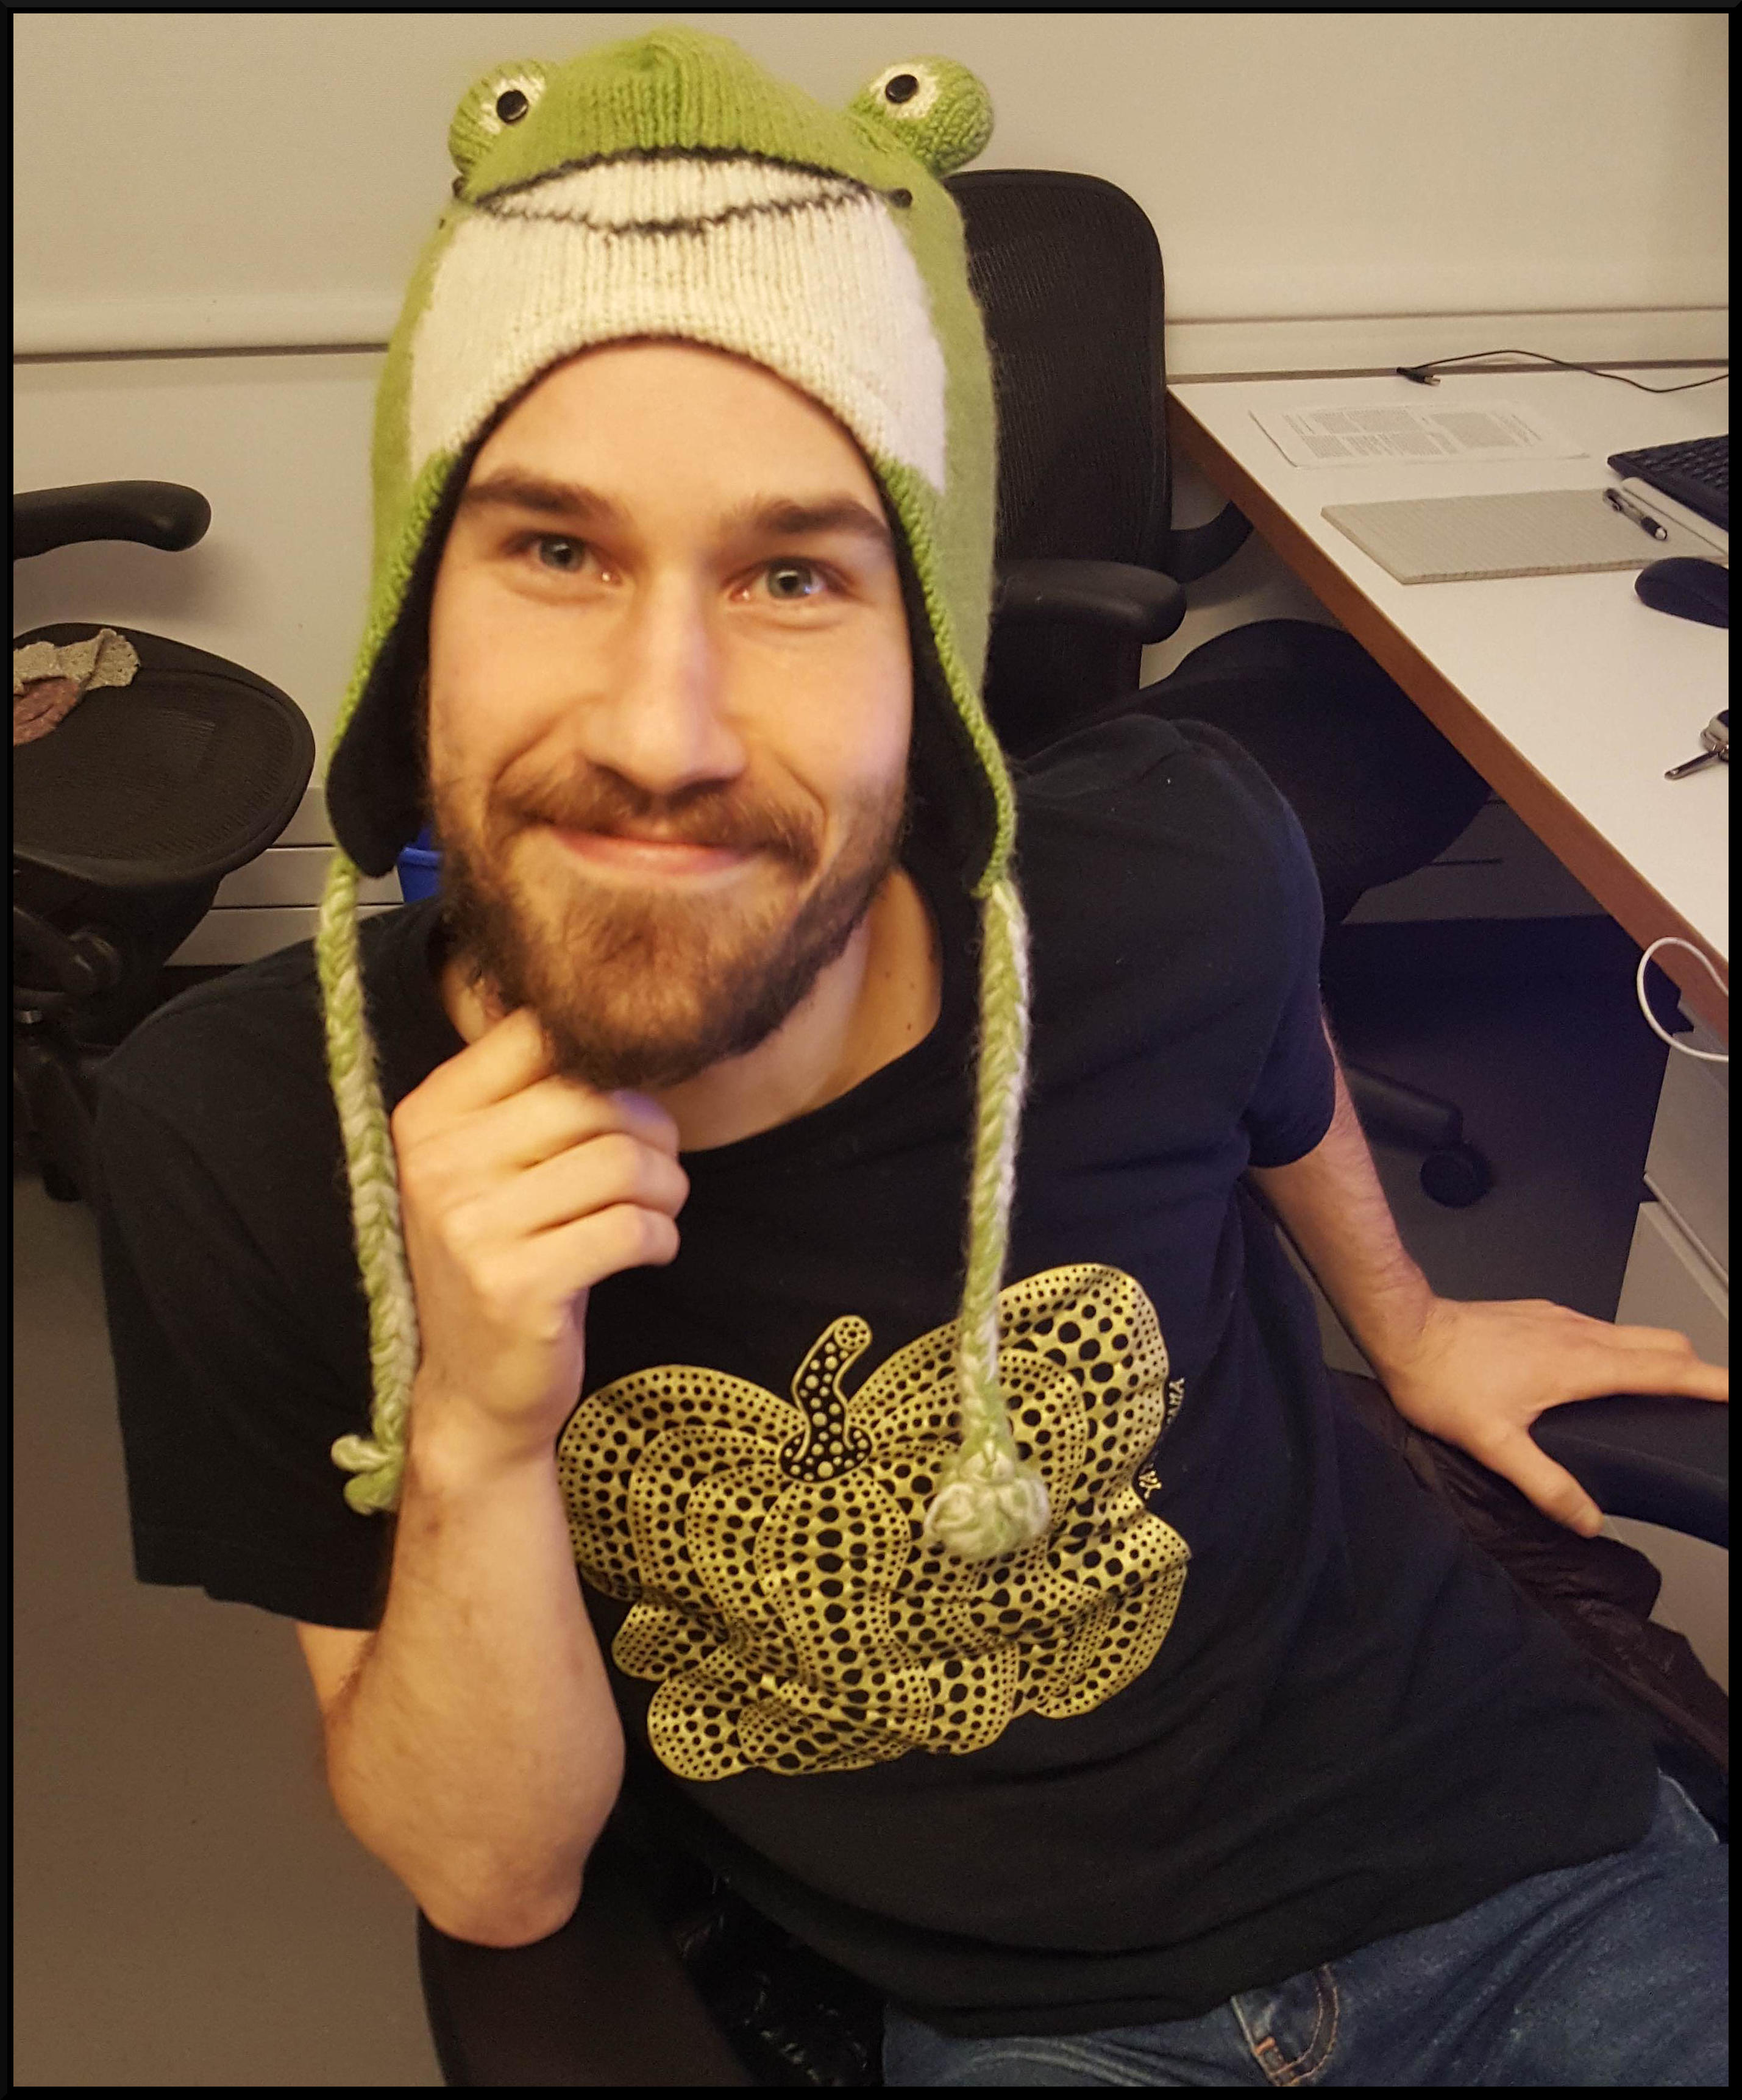
\includegraphics[height=2.60417in]{/assets/images/LewallenSam.jpg}

Sam Lewallen

\begin{itemize}
\tightlist
\item
  \href{/pdf/cv_lewallen_WEB.pdf}{\emph{}}
\item
  \href{https://scholar.google.com/citations?user=f17bjxcAAAAJ\&hl=en}{\emph{}}
\item
  \href{https://mathoverflow.net/users/492/sam-lewallen}{\emph{}}
\end{itemize}

\href{mailto:slewallen@fas.harvard.edu}{\nolinkurl{slewallen@fas.harvard.edu}}

Click \href{https://compneurojc.github.io}{HERE}\\
for MIT/Harvard computational\\
neuroscience journal club

\hypertarget{contextbox}{}
\subsection{About}\label{about}

\begin{center}\rule{0.5\linewidth}{\linethickness}\end{center}

I'm a theoretical neuroscientist, with a background in pure mathematics.
I'm currently a
\href{http://cbs.fas.harvard.edu/science/swartz-program}{Swartz fellow}
at Harvard University in the \href{http://cbs.fas.harvard.edu}{Center
for Brain Science}.

\subsection{Publications}\label{publications}

\begin{center}\rule{0.5\linewidth}{\linethickness}\end{center}

\hypertarget{publications}{}
Probing variability in a cognitive map using manifold inference from
neural dynamics

Ryan J Low*, Sam Lewallen*, Dmitriy Aronov, Rhino Nevers, David W Tank
(2018). \emph{bioRxiv}.

\begin{itemize}
\tightlist
\item
  \href{https://www.biorxiv.org/content/early/2018/09/20/418939}{\emph{}}
\item
  \href{/pdf/Low_Lewallen_et_al_2018_Probing_variability_in_a_cognitive_map_using_manifold_inference_from_neural.pdf}{\emph{}}
\end{itemize}

A map-like micro-organization of grid cells in the medial entorhinal
cortex

Yi Gu, Sam Lewallen, Amina A Kinkhabwala, Cristina Domnisoru, Kijung
Yoon, Jeffrey L Gauthier, Ila R Fiete, David W Tank (2018). \emph{Cell}.

\begin{itemize}
\tightlist
\item
  \href{https://www.sciencedirect.com/science/article/pii/S009286741831167X}{\emph{}}
\item
  \href{/pdf/Gu_et_al_2018_A_Map-like_Micro-Organization_of_Grid_Cells_in_the_Medial_Entorhinal_Cortex.pdf}{\emph{}}
\end{itemize}

Grid cell responses in 1D environments assessed as slices through a 2D
lattice

KiJung Yoon*, Sam Lewallen*, Amina A Kinkhabwala, David W Tank, Ila R
Fiete (2016). \emph{Neuron}.

\begin{itemize}
\tightlist
\item
  \href{https://www.sciencedirect.com/science/article/pii/S0896627316000647}{\emph{}}
\item
  \href{/pdf/Yoon_et_al_2016_Grid_Cell_Responses_in_1D_Environments_Assessed_as_Slices.pdf}{\emph{}}
\end{itemize}

Stimulus-dependent correlations in threshold-crossing spiking neurons

Yoram Burak, Sam Lewallen, Haim Sompolinsky (2009). \emph{Neural
Computation}.

\begin{itemize}
\tightlist
\item
  \href{https://arxiv.org/abs/0902.2037}{\emph{}}
\item
  \href{https://www.mitpressjournals.org/doi/abs/10.1162/neco.2009.07-08-830}{\emph{}}
\item
  \href{/pdf/Burak_et_al_2009_Stimulus-dependent_correlations_in_threshold-crossing.pdf}{\emph{}}
\end{itemize}

(1,1) L-space knots

Joshua Evan Greene, Sam Lewallen, Faramarz Vafaee** (2018).
\emph{Compositio Mathematica}.

\begin{itemize}
\tightlist
\item
  \href{https://arxiv.org/abs/1610.04810}{\emph{}}
\item
  \href{https://www.cambridge.org/core/journals/compositio-mathematica/article/11-lspace-knots/913FE639D9C8D4BDDFBC6F23AD9A7488\#}{\emph{}}
\item
  \href{/pdf/Greene_et_al_2018_$(1,1)$_L-space_knots.pdf}{\emph{}}
\end{itemize}

Strong L-spaces and left orderability

Adam Simon Levine, Sam Lewallen** (2012). \emph{Mathematical Research
Letters}.

\begin{itemize}
\tightlist
\item
  \href{https://arxiv.org/abs/1110.0563}{\emph{}}
\item
  \href{https://www.intlpress.com/site/pub/pages/journals/items/mrl/content/vols/0019/0006/a005/}{\emph{}}
\item
  \href{/pdf/Levine_Lewallen_2012_Strong_L-spaces_and_left-orderability.pdf}{\emph{}}
\end{itemize}

* Joint first authors\\
** Authors in alphabetical order

\subsection{Theses}\label{theses}

\begin{center}\rule{0.5\linewidth}{\linethickness}\end{center}

\hypertarget{publications}{}
Floergåsbord

Phd thesis

\begin{itemize}
\tightlist
\item
  \href{/pdf/Floergasbord.pdf}{\emph{}}
\end{itemize}

The volume conjecture

Undergraduate thesis

\begin{itemize}
\tightlist
\item
  \href{/pdf/volume_conjecture.pdf}{\emph{}}
\end{itemize}




\end{document}